\documentclass[11pt,a5paper]{article}

\usepackage[T1]{fontenc}
\usepackage[utf8]{inputenc}
\usepackage{lmodern, microtype}
\usepackage[estonian]{babel}
\usepackage{siunitx}
\sisetup{inter-unit-product=\ensuremath{{\cdot}}, per-mode=fraction, exponent-product=\cdot, output-decimal-marker={,}}
\usepackage{graphicx}
\usepackage{wrapfig}
\usepackage{adjustbox}
\usepackage{amsmath,amssymb}
\usepackage{amsfonts}
\usepackage[hidelinks]{hyperref}
\usepackage{csquotes}
\usepackage{caption}
\usepackage{enumitem}
\usepackage{soulutf8}
\topmargin=-3.0cm \textheight=19cm \textwidth=12.9cm
\oddsidemargin=-1.5cm  \evensidemargin=-1.5cm
\setlength{\parindent}{0pt} \setlength{\parskip}{6pt} \sloppy
\sloppy \relpenalty=10000 \binoppenalty=10000
\pagestyle{empty}

\newcommand{\numb}[1]{\vspace{5pt}\textbf{\large #1}}
\newcommand{\nimi}[1]{(\textsl{\small #1})}
\newcommand{\punktid}[1]{(\emph{#1~p.})}
\newcounter{ylesanne}
\newcounter{expylesanne}
\newcommand{\yl}[1]{\addtocounter{ylesanne}{1}\numb{\theylesanne.} \nimi{#1} \newblock{}}
\newcommand{\expyl}[1]{\addtocounter{expylesanne}{1}\numb{E\theexpylesanne.} \nimi{#1} \newblock{}}
\newcommand{\autor}[1]{}% Kasuta võistluse ajal
%\newcommand{\autor}[1]{\emph{Autor: #1}}% Kasuta kui vaja autorit

\begin{document}
\begin{center}
  \textbf{\Large Eesti koolinoorte 70. füüsikaolümpiaad} \par
  \emph{10. veebruar 2023. a. Piirkondlik voor.\\Gümnaasiumi ülesanded (10.--12. klass)}
\end{center}

\resizebox{\textwidth}{!}{
  \emph{%
    \begin{tabular}{@{}l@{}}
      \textbf{Palun kirjutada iga ülesande lahendus eraldi lehele.}\\
      Lahendamisaeg on 5 tundi. \\
      Iga osavõtja võib lahendada kõiki pakutud ülesandeid. \\
      Arvesse lähevad 5 suurima punktide arvu saanud teoreetilist ja 1 eksperimentaalne ülesanne. \\
      Kasutada võib kirjutus- ja joonestusvahendeid ning kalkulaatorit. Muud abivahendid on keelatud.\\
      Eksperimentaalülesande lahendamisel võib kasutada üksnes loetelus toodud vahendeid. \\
      Mõõtemääramatuse hindamist ei nõuta.
    \end{tabular}
  }
} \par


\yl{VALGUSVIHK} Maril on taskulamp, millest väljub paralleelne valgusvihk diameetriga $\SI{30}{\mm}$. Et koondada lambist tulenev valgus eredamaks, soovib Mari läätsede abil muuta valgusvihu väiksemaks paralleelseks valgusvihuks diameetriga $\SI{5}{\mm}$. Mari tuhnib oma sahtlis ringi ning leiab, et tal on nii kumer- kui nõgusläätsed järgnevate fookuskaugustega: $\SI{1}{\cm}$, $\SI{2}{\cm}$, $\SI{3}{\cm}$, $\SI{5}{\cm}$, $\SI{8}{\cm}$, $\SI{10}{\cm}$, $\SI{12}{\cm}$ ja $\SI{15}{\cm}$. Leidke, kuidas ja milliste fookuskaugustega läätsede abil on Maril võimalik oma eesmärk saavutada, kasutades
\\ (a) kaht kumerläätse.
\\ (b) üht kumerläätse ja üht nõgusläätse.
\\ Kummalgi juhul joonistage skeem.
\punktid{6} \autor{Richard Luhtaru}

\yl{OTSENE KALORIMEETRIA}
Üks viis, kuidas mõõta inimeselt või loomalt eralduva soojuse võimsust, on otsene kalorimeetria. Selle käigus pannakse inimene soojusisolatsiooniga tuppa, kus tagatakse inimese jaoks vajalik õhuvahetus. Kehast eralduva soojushulga leidmiseks läbib tuba veetoru, milles oleva vee temperatuur mõõdetakse enne ja pärast toa läbimist. Eeldage, et vesi siseneb tuppa temperatuuril $T_1 = \SI{20.00}{\celsius}$ ning väljub temperatuuril $T_2 = \SI{20.15}{\celsius}$. Vee kiirus torus on $u = \SI{2}{\meter\per\second}$ ja toru ristlõikepindala on $S=\SI{1}{\cm\squared}$. Mis on inimese kehast eralduva soojuse võimsus $P$? Vee tihedus on $\rho = \SI{1000}{\kg\per\meter\cubed}$ ning vee erisoojus on $c = \SI{4200}{\joule\per\kilogram\per\celsius}$. Võib eeldada, et õhuvahetuse käigus soojusvahetust ei toimu ning süsteem on termodünaamilises tasakaalus.
\punktid{6} \autor{Konstantin Dukatš}
%(NB! Vana versiooni tõlge, eestikeelne tekst on uuendatud) Одним из способов определения количества тепла, выделенного организмом человека или животного является прямая калориметрия. Представим, что человека поместили в теплоизолированную комнату, в которую подается О$_2$ и поглощается избыток СО$_2$ и водяных паров. Продуцируемое организмом человека тепло измеряют с помощью термометров по нагреванию воды, протекающей по трубкам в камере. Вода температуры $T_1 = 20.00 \degree C $ входит в камеру, а выходит с температурой $T_2 = 20.15 \degree C $. Высота между поверхностью воды в бассейне до входа в камеру и краном после выхода постоянна и равна $h = 0.2$m, площадь поперечного сечения трубы $S=1$ cm$^2$. Чему равна мощность $P$ выделения тепла человеком? 

\yl{ÖKONOOMNE SÕIT}
Linnas kiirendab sisepõlemismootoriga auto tippkiiruseni $\SI{40}{\km\per\hour}$ ning peab peatuma keskmiselt iga $100$ meetri tagant. Linnasõidul võib õhutakistust mitte arvestada. Maanteel sõidab auto püsiva kiirusega $\SI{90}{\km\per\hour}$. Õhutakistusjõud avaldub kujul $F=cv^2$, kus $c = \SI{1.3}{\kg\per\meter}$ ja $v$ on auto kiirus. Auto kaalub $\num{1.5}$ tonni. Leidke maanteesõidu ja linnasõidu kütusekulude suhe $\SI{100}{\km}$ sõidu kohta. Eeldage, et mootori kasutegur ei sõltu kiirusest ja kiirendusest.
\punktid{8} \autor{Marten Rannut}

\yl{DROON}
Droon massiga $m=\SI{500}\g$ hõljub õhus ja püsib paigal. Äkitselt hakkab puhuma järjest tugevnev tuuleiil ning selleks, et drooni paigal hoida, käivituvad drooni horisontaalsuunas tõukavad propellerid. On teada, et tuule poolt droonile mõjuv horisontaalsuunaline jõud kasvab konstantse kiirusega nullist puhangu alguses kuni väärtuseni $F_t=\SI{25}\N$ ajahetkel $t_t= \SI{0.7}\s$. Drooni horisontaalsuunalist liikumist kontrollivad propellerid avaldavad tõukejõudu, mis kasvab samuti konstantse kiirusega, nullist puhangu alguses kuni väärtuseni $F_p=\SI{20}\N$ ajahetkel $t_p= \SI{1.0}\s$. Leidke drooni horisontaalsuunaline kiirus $t=\SI{0.5}\s$ pärast puhangu algust.
\punktid{8} \autor{Marten Rannut}

\begin{wrapfigure}{r}{0.3\textwidth}
  \vspace{-2em}
  \begin{center}
    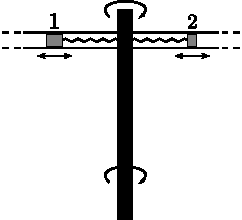
\includegraphics[width=1\linewidth]{vedru_keerutamine_joonis.pdf}
  \end{center}
  \vspace{-2em}
\end{wrapfigure}

\yl{VEDRU KEERUTAMINE}
Kaks erineva jäikusega, kuid sama pikkusega vedru on kinnitatud ühest otsast posti külge. Kummagi vedru teises otsas on raskus, kusjuures esimese vedru otsas olev raskus on kaks korda suurema massiga kui teise vedru otsas olev raskus. Mõlemad vedrud asuvad hõõrdevabas kanalis, kus raskused saavad liikuda ainult horisontaalselt, mistõttu gravitatsiooniga arvestama ei pea. Post hakkab pöörlema nii, et ka vedrude otsas olevad massid hakkavad liikuma ringsel trajektooril. Selle peale pikeneb esimene vedru kaks korda ja teine neli korda. Mis on vedrude jäikuste suhe? Vedrude enda massid võib lugeda raskuse massiga võrreldes tühiselt väikeseks. Eeldage, et vedru pikenemine on piisavalt väike selleks, et kehtiks Hooke'i seadus.
\punktid{8} \autor{Sandra Schumann}

\begin{wrapfigure}{r}{0.3\textwidth}
  \vspace{-2em}
  \begin{center}
    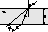
\includegraphics[width=1\linewidth]{klaasplaat_joonis.pdf}
    %\caption{}
  \end{center}
  \vspace{-2em}
\end{wrapfigure}

\yl{KLAASPLAAT}
Leidke, kui palju nihkub valguskiir kõrvale esialgse sihi suhtes pärast klaasplaadi läbimist. Kiire langemisnurk on $\alpha$, klaasi murdumisnäitaja on $n$ ning klaasplaadi paksus on $d$. Täispunktide saamiseks palume vastuses mitte kasutada trigonomeetrilisi pöördfunktsioone (nt $\arcsin$, $\arccos$).
\punktid{10} \autor{Erkki Tempel}

\begin{wrapfigure}{r}{0.35\textwidth}
  \begin{center}
    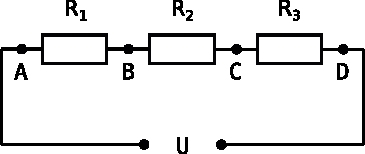
\includegraphics[width=1\linewidth]{ahelad_efo.pdf}
  \end{center}
  \vspace{-2em}
\end{wrapfigure}

\yl{VOLTMEETER}
Kolm tundmatut takistit on ühendatud jadamisi ja neile on rakendatud pinge $U=\SI{126}{\volt}$. Tundmatu sisetakistusega voltmeetriga mõõdetakse pingeid joonisel näidatud punktide vahel. Tulemuseks on näidud $V_{AB}=V_{CD}=\SI{28}{\volt}$ ja $V_{AC}=\SI{84}{\volt}$. Millist pinget näitab voltmeeter, kui selle klemmid ühendada punktidega B ja C?
\punktid{10} \autor{Päivo Simson}

\newpage

\begin{wrapfigure}{r}{0.35\textwidth}
\vspace{-1em}
  \begin{center}
    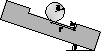
\includegraphics[width=1\linewidth]{syvend_kera_joonis.pdf}
  \end{center}
  \vspace{-2em}
\end{wrapfigure}

\yl{SÜVEND JA KERA}
Tasandil on silindrikujuline süvend raadiusega $r$ ning sügavusega $h$, mis on risti tasandi pinnaga. Süvendi sisse asetatakse kera raadiusega $R$, nii et kera puudutab süvendi keskpunkti ja kera on algselt paigal. Tasand on maapinna suhtes kaldus nurga $\theta$ võrra. Millist tingimust peavad rahuldama antud suurused, et kera saaks mingi arvu põrgete järel süvendist välja hüpata? Võib eeldada, et hõõrdumist ei toimu, põrked on täielikult elastsed, pindade ebatasasuste tõttu on põrkesuunad vähesel määral juhuslikud ning $h < R$.
\punktid{10} \autor{Marko Tsengov}

\yl{SÜGAV KAEV}
Kilplased ehitasid umbes 11 meetri sügavuse pumbakaevu. Lihtsustatult võime nende kaevu vaadelda kui pikka vertikaalset silindrilist toru, mille ülaotsas tekitab pump alarõhu ja imeb seeläbi vett ülespoole. Toru alumine ots on lahtine: vesi saab sealt vabalt nii sisse kui välja voolata. Kilplased proovisid hommikul vett pumbata --- pumpasid ja pumpasid, aga pumbatoru ülemisest otsast jäi veetase ikka umbes meetri kaugusele.  Nad väsisid ära ja läksid puhkama. Peale paaritunnist puhkust tulid tagasi ja proovisid uuesti, aga nüüd jäi  veetase pumbatoru ülemisest otsast veel kaugemale. Mitme sentimeetri võrra jäi veetase teisel katsel madalamaks? On teada, et õhus oli vett nii enne kui pärast $\rho_a=\SI{8}{\g\per\m\cubed}$, aga et õhk oli soojenenud hommikuselt $T_1=\SI{10}{\celsius}$ väärtuseni $T_2=\SI{20}{\celsius}$, siis suhteline õhuniiskus oli vähenenud $r_1=80\%$-lt $r_2=40\%$-ni. Vee tihedus on $\rho_v=\SI{1000}{\kg\per\m\cubed}$ ja molaarmass $\mu=\SI{18}{\g\per\mol}$, gaasikonstant $R=\SI{8.31}{\joule\per\kelvin\per\mol}$, vabalangemise kiirendus $g=\SI{9.8}{\m\per\s\squared}$. Eeldage, et vee temperatuur torus on võrdne õhutemperatuuriga ning õhurõhk päeva jooksul ei muutunud.
\punktid{12} \autor{Jaan Kalda}

\yl{ALAJAAMA KAUGUS}
Maja peakaitsmeni tuuakse elektrivool alajaamast jämeda alumiiniumist juhtmepaari abil, millest üks, nn nulljuhe, on maandatud alajaama juures. Mõlemad juhtmed on ühepikkused ja ühesuguse ristlõike pindalaga $S=\SI{35}{\mm\squared}$. Alumiiniumi eritakistus on $\rho=\SI{2.7e-8}{\ohm\m}$. Tegemist on elektriliini kõige alajaamapoolsema tarbimispunktiga --- elektriliin jätkub järgmiste majapidamiste poole. Maja sees on elektri edasi kandmiseks peenemad sinist ja pruuni värvi juhtmed, mis on peakaitsmes ühendatud alajaamast tulevate juhtmete külge: sinine on ühendatud nulljuhtmega ja pruun võrgupinget kandva nn faasijuhtmega. Peale selle saab peakaitsme juurest alguse sealsamas maandatud rohe-kollane maandusjuhe. Maandamine tagab selle, et juhe omab maapinna elektrilist potentsiaali (kui juhtmes on elektrivool, siis kehtib see vaid maanduspunkti lähedal; maandusjuhtmes voolu ei ole). Et maapind on hea elektrijuht, siis on maapinna potentsiaal kõikjal üks ja sama. 

Kui majas on sisse lülitud  elektriradiaator, siis on maja peakaitsme juures pinge sinise ja kolla-rohelise juhtme vahel $U_1=\SI{30}\V$  ning sinise ja pruuni vahel $U_f=\SI{210}\V$. Radiaatori nominaalpinge on $U_n=\SI{230}\V$ ja nominaalvõimsus on $P_n=\SI 2{\kW}$ (st kui radiaatorile rakendatakse nominaalpinge, siis eraldub radiaatoril nominaalvõimsus). Radiaatori välja lülitamisel väheneb rohe-kollase juhtme ja sinise juhtme vaheline pinge väärtuseni $U_0=\SI{20}\V$. Kui pikk on majast alajaamani viiv juhtmepaar? Eeldage, et nii radiaatorit kui ka elektriliinil paiknevaid teisi tarbijaid võib heas lähenduses vaadelda kui takisteid. Muuhulgas tähendab see, et kuigi võrgus on vahelduvpinge, võib arvutusi teha täpselt samamoodi nagu alalispinge puhul.
\punktid{12} \autor{Jaan Kalda}

\end{document}